\section{Cornerstone}
\label{sec:cornerstone}

To characterize Cornerstone's performance we first need to understand the algorithmic steps. Note that there are two methods of interest, the method where an octree is constructed locally on a node and the case where a locally essential tree is used for distributed simulation. We review the local case first and then advance to the distributed case as an extension. We focus primarily on the steps needed and how they map to GPU architectures, for further insight to the algorithm reference Cornerstone ~\cite{cornerstone}. An outline of the steps in construction is given for the local case.
\begin{itemize}
    \item Compute a space filling curve (Morton or Hilbert)
    \item Sort the keys and rearrange any properties associated with the key such as the position, mass, charge, etc
    \item Update the leaf nodes
    \item Update the internal tree structure
\end{itemize}

Additionally Cornerstone has 6 critical parameters which are tabulated below to give an overview. These will also be important parameters for characterization.

\begin{table}[h!]
    \centering
    \caption{Cornerstone Parameters}
    \label{tab:my_table}
    \begin{tabular}{|c|c|c|}
        \hline
        \textbf{Parameter} & \textbf{Description} \\
        \hline
        Precision & FP64 or FP32 \\
        $\theta$ & The MAC parameter \\
        $N_{crit}$ & Maximal \# of points in a leaf \\ 
        $h$ & Smoothing parameter \\
        $L$ & The maximal depth of the octree \\
        SFC & Morton or Hilbert \\
        \hline
    \end{tabular}
\end{table}

\subsection{Space Filling Curves}

Informally a space filling curve will take points existing in space and map them to integer keys, when one sorts the original particles based on these keys and traverses the path through them the resulting curve will recursively move through the domain octant by octant (in the case of three dimensional points). In this way a space filling curve is a kind of fractal.

We are interested in two types of space filling curves namely Morton Z-order curves and Hilbert curves. The path of a Morton Z-order curve may be viewed in figure \ref{fig:morton_leaves} and shows the distinct z-pattern. Morton codes are computationally efficient to calculate requiring just a few bit shifts, but as is also evident visually in figure \ref{fig:morton_leaves} the curve may "jump" octants resulting in unfavorable communication patterns between nodes.

The Hilbert curve on the other hand takes on a compact U shape as seen in figure \ref{fig:hilbert_leaves}. Hilbert codes offer a "compact" mapping which may reduce the cost of communication but come at the cost in increased computational inefficiency requiring $L$ loop iterations, $L$ being the maximal depth of the octree.

\begin{figure}[h!]
    \centering
    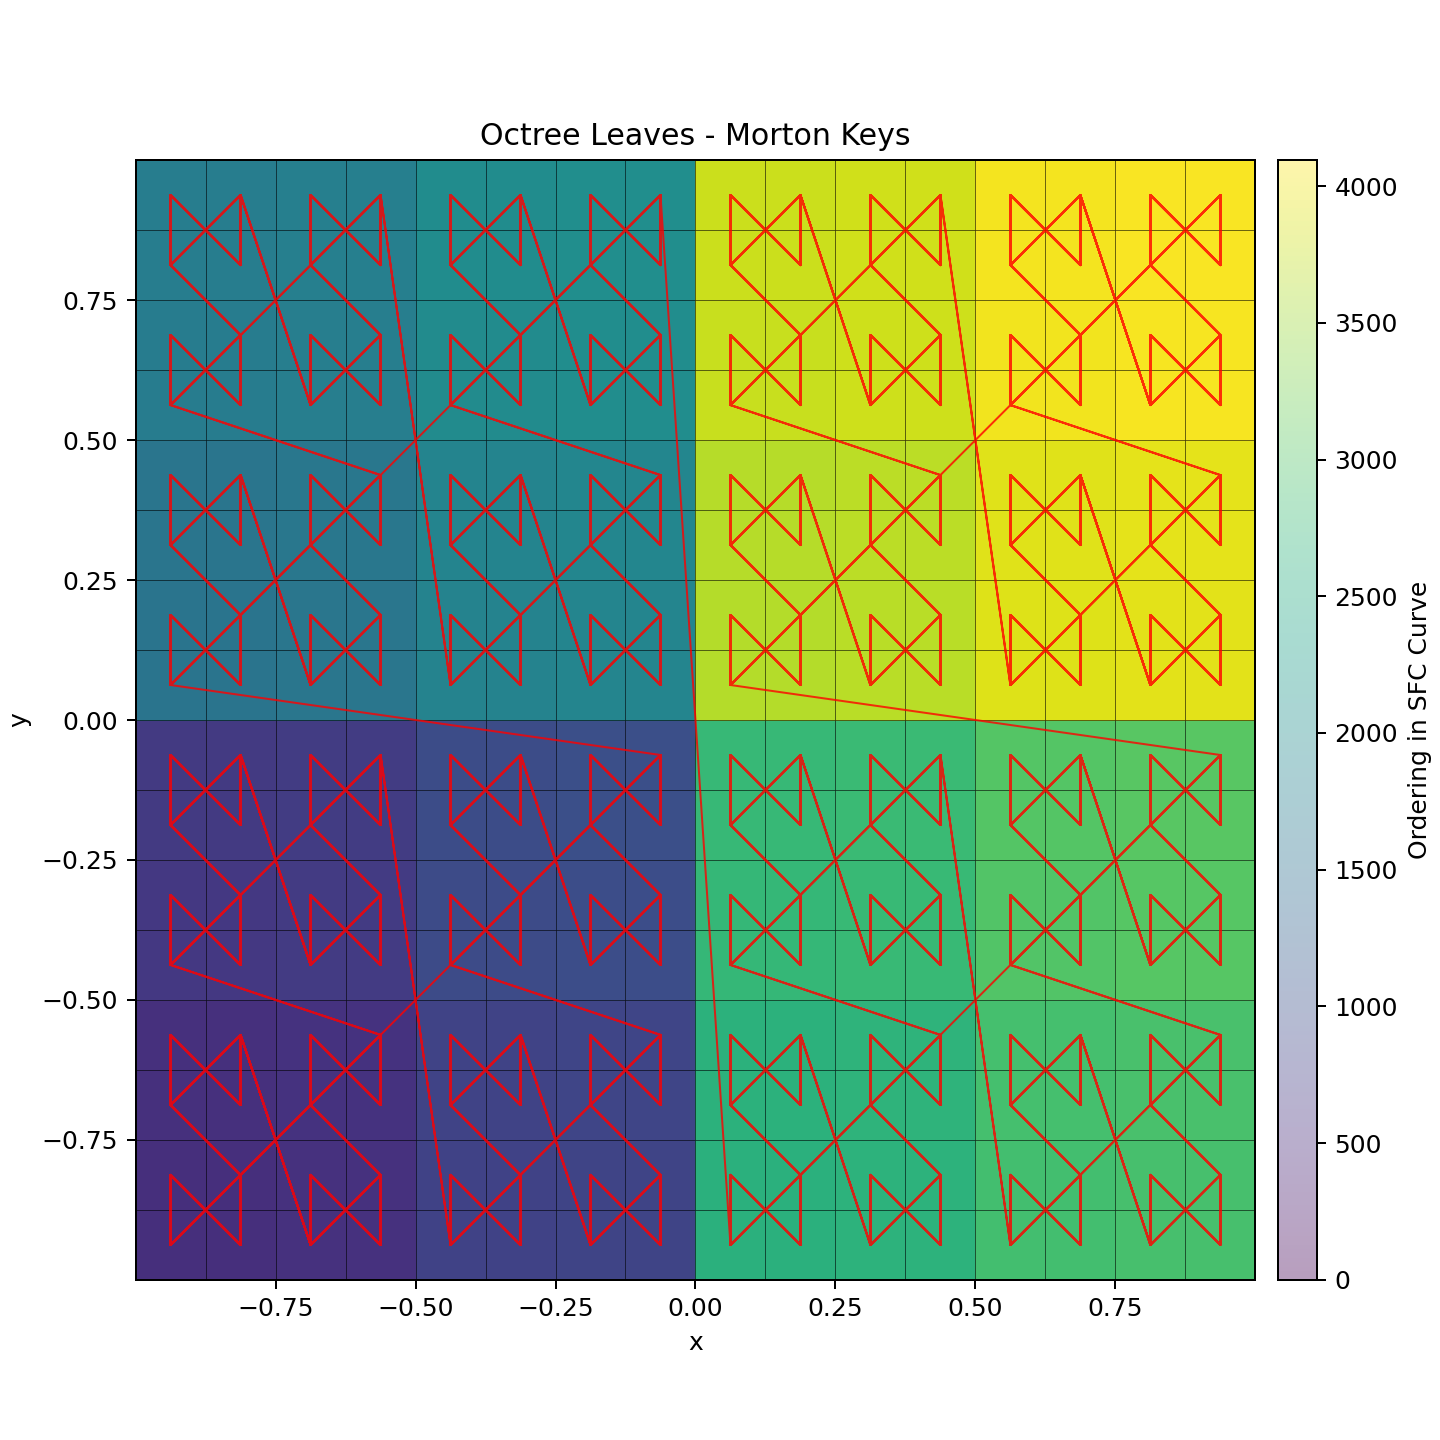
\includegraphics[width=0.45\textwidth]{assets/leaves_morton.png}
    \caption{The leaves of an octree colored with respect to their Morton Z-order curve. The red trace plots the curves path through the leaves.}
    \label{fig:morton_leaves}
\end{figure}

\begin{figure}[h!]
    \centering
    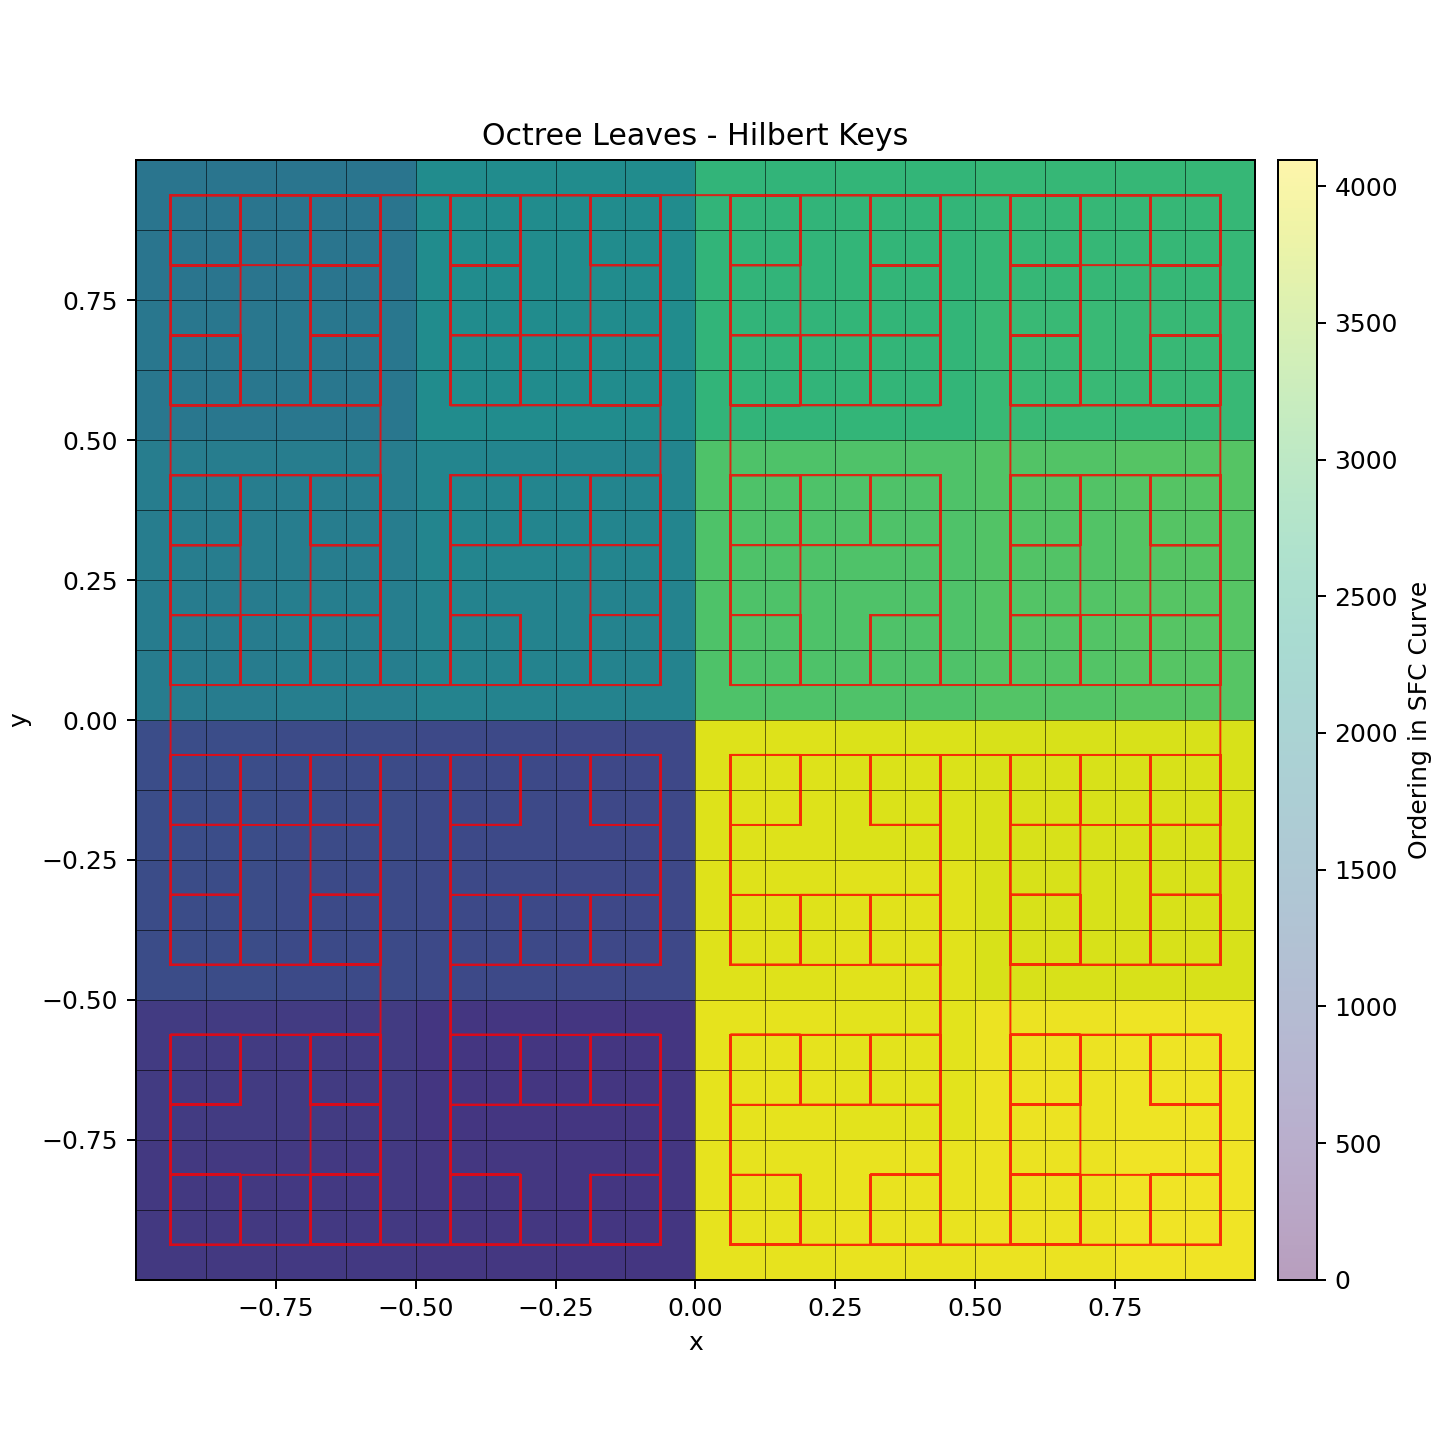
\includegraphics[width=0.45\textwidth]{assets/leaves_hilbert.png}
    \caption{The leaves of an octree colored with respect to their Hilbert curve. The red trace plots the Hilbert curve path through the leaves.}
    \label{fig:hilbert_leaves}
\end{figure}

\subsection{Radix Sorting and Gathers}
We will not detail the Radix sort and Gather implementations as they are well known. The reason these operations are necessary is to sort the keys thus producing the in-order arrangement of keys according to the space filling curve that recursively partitions the space into octants. The keys will have some attributes including $x,y,z$ but may have others based on the application, these also need to be aligned with the sorted keys. In Cornerstone these are distinct kernels with an Radix sort and $k$ gathers for the number of properties to be sorted.

\subsection{Update Leaf Nodes}
The namesake of Cornerstone ~\cite{cornerstone} is the Cornerstone array called $K$. $K$ is a sorted array of SFC keys of length $n_l+1$, $n_l$ being the number of leaves, with the first element being $0$ and the last element being $8^L$, with the difference between one element and it's successor being $8^l$, where $l \le L$. Then $K$ will define a unique octree but represents explicitly the leaves. Then the steps to generate the Cornerstone array from the particle SFCs are to calculate a histogram of the particle SFCs belonging to each each leaf node and then perform three steps:
\begin{enumerate}
    \item Compute the rebalancing decision for each node i.e a code where 8 indicates $N_{crit} < N_i$ and so the node should be subdivided, 0 indicates the node should be replaced, and 1 indicates the leaf should be unchanged.
    \item Perform an exclusive prefix sum of the array of computed rebalancing decision codes, this leads to each element in the result being the new index of the node in the corresponding new Cornerstone array. The final element is the number of nodes in the new Cornerstone array.
    \item Finally if the rebalancing decision for node $i$ is $1$ then the key is copied to the new index calculated in the exclusive prefix sum. If the decision is to split, the code is $8$ and we copy the keys of the children of the original node to the new range.
\end{enumerate}
A Cornerstone array is then balanced once no node needs to be split or merged, which means that every leaf node has a particle count $\le N_{crit}$ and every internal node has a particle count $> N_{crit}$. By iteratively applying these steps until we reach the criteria for a balanced Cornerstone array we define a balanced octree.

Regarding performance, note that each kernel launch here must occur in serial, no stream parallelism is possible or kernel fusion. Additionally a memory allocation is necessary and has to read the value of the last element of the exclusive prefix sum to calculate the number of new leaf nodes. 

\subsection{Update Internal Nodes}
Finally the internal tree structure must be created allowing us to traverse the tree and ultimately we are left with three arrays of integers, note $n = n_i + n_l$ with $n_i$ being the number of internal nodes and $n_l$ being the number of leaf nodes:
\begin{enumerate}
    \item $NK$ of size $n$, with each value being within the range defined by the SFC size supported by $L$ which is $[0,2^{3L})$. This is the SFC key for each node both leaves and internal.
    \item $CO$ of size $n$, with each value being in the range $[1,n)$. This is the connectivity array.
    \item $LO$ of size $L + 2$ with each value being in the range $[1,n)$ which are the tree level offsets.
\end{enumerate}

